\documentclass[crop,tikz]{standalone}
\usetikzlibrary{backgrounds}
\colorlet{blue}{cyan}
\tikzset{
  inverted/.style = {
    color=white,
    background rectangle/.style={fill},
    show background rectangle
  }
}

\tikzset{>=latex}
\usetikzlibrary{decorations.markings}
\colorlet{green}{green}
\definecolor{orange}{RGB}{250,194,25}
\newcommand{\place}{\vec{r}}
\newcommand{\velocity}{\vec{v}}
\newcommand{\acceleration}{\vec{a}}

\begin{document}
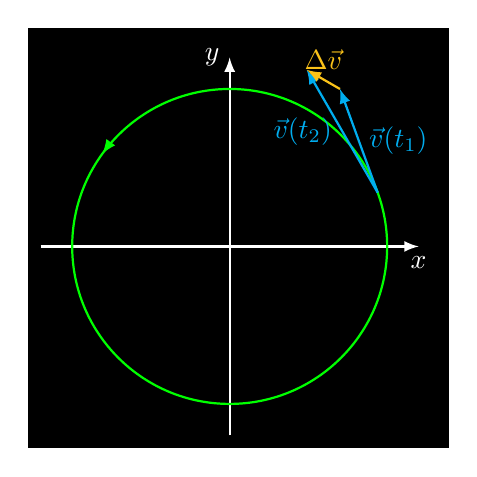
\begin{tikzpicture}[inverted,scale=2]
  % axes
  \draw[->,thick] (-1.2,0) -- (1.2,0) node[below] {$x$};
  \draw[->,thick] (0,-1.2) -- (0,1.2) node[left] {$y$};
  % circle
  \draw[
    decoration={markings, mark=at position 0.4 with {\arrow{>}}},
    postaction={decorate},
    green,
    thick
  ] (0,0) circle (1);
  % place, velocity
  \draw[->,thick,blue] (20:1) -- node[right]{$\velocity(t_1)$} ++(20+90:0.7) coordinate (v1);
  % place, velocity
  \draw[->,thick,blue] (20:1) -- node[left]{$\velocity(t_2)$} ++(30+90:0.9) coordinate (v2);
  \draw[->,thick,orange] (v1) -- node[above] {$\Delta\velocity$} (v2);
\end{tikzpicture}
\end{document}
